\documentclass{article}
\usepackage[utf8]{inputenc}
\usepackage[greek,english]{babel}
\usepackage{alphabeta}
\usepackage{graphicx}
\usepackage{amsmath}
\usepackage{hyperref}
\usepackage{longtable}
\usepackage{geometry}
\usepackage{listings}
\geometry{a4paper, margin=1in}
\usepackage{textgreek}

\title{Ιόνιο Πανεπιστήμιο, Τμήμα Πληροφορικής}
\author{Σταμάτης Πέτρου AM:inf2021186 , Παύλος - Μάριος Γιαννάκος AM:inf2021040}

\begin{document}
\maketitle

\section{Εισαγωγή}
Αυτή η αναφορά περιγράφει την ανάλυση ενός συνόλου δεδομένων (Βαθμοί οδηγών ανά αγώνα, χρόνοι γύρων κάθε οδηγού για κάθε πίστα, χρόνοι pit stop του κάθε οδηγού σε κάθε αγώνα, ελαστικά που χρησιμοποιήθηκαν κλπ) Formula 1 χρησιμοποιώντας Python. Η εφαρμογή χτίστηκε χρησιμοποιώντας Streamlit, επιτρέποντας διαδραστική απεικόνιση δεδομένων μέσω μηχανικής μάθησης.

\section{Σχεδιασμός Εφαρμογής}
Η εφαρμογή σχεδιάστηκε με σκοπό να παρέχει έναν εύχρηστο τρόπο ανάλυσης και απεικόνισης των δεδομένων Formula 1. Χρησιμοποιήθηκαν οι παρακάτω τεχνολογίες:
\begin{itemize}
    \item Python
    \item Βιβλιοθήκες: pandas, numpy, matplotlib, seaborn, scikit-learn
    \item Streamlit για τη δημιουργία του διαδραστικού περιβάλλοντος
\end{itemize}

\section{Υλοποίηση}
\textbf{Η υλοποίηση περιλαμβάνει τα ακόλουθα στάδια:}
\subsection{Φόρτωση και Επεξεργασία Δεδομένων}
Τα δεδομένα φορτώθηκαν από ένα αρχείο CSV και προεπεξεργάστηκαν για να αφαιρεθούν τυχόν ελλιπείς ή μη χρήσιμες πληροφορίες.

\subsection{Απεικόνιση Δεδομένων}
Οι απεικονίσεις των δεδομένων πραγματοποιήθηκαν χρησιμοποιώντας PCA (Κύρια Συνιστώσα Ανάλυση) και t-SNE (t-κατανεμημένη Στοχαστική Ενσωμάτωση Γειτόνων).

\subsection{PCA Visualization}
Το PCA χρησιμοποιήθηκε για τη μείωση των διαστάσεων των δεδομένων σε δύο συνιστώσες. Το PCA χρησιμοποιήθηκε για την απεικόνιση και για να οπτικοποιηθεί η κατανομή των δεδομένων. Παρακάτω είναι το διάγραμμα διασποράς του PCA:

\begin{figure}[h]
    \centering
    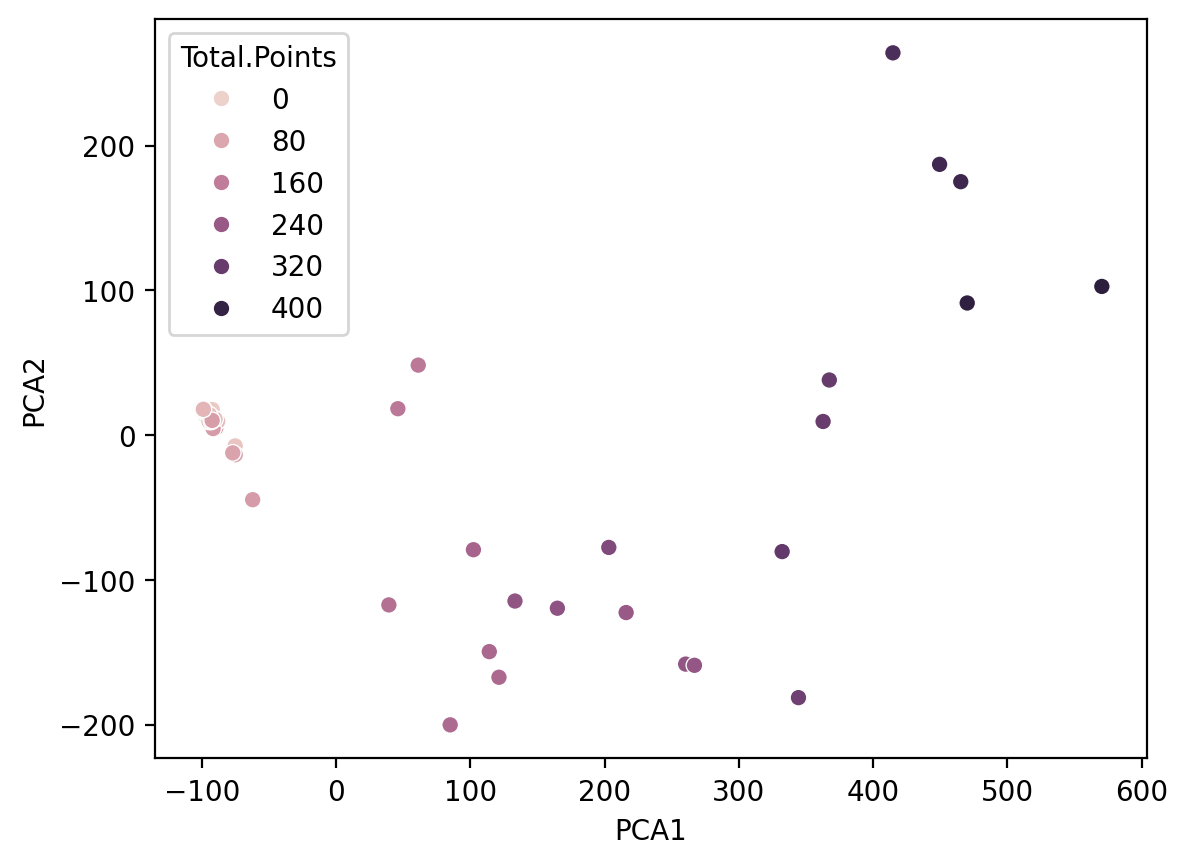
\includegraphics[width=\textwidth]{pca_plot.png} 
    \caption{Διάγραμμα Διασποράς PCA}
    \label{fig:pca}
\end{figure}

\subsection{t-SNE Visualization}
Το t-SNE χρησιμοποιήθηκε επίσης για τη μείωση των διαστάσεων και την απεικόνιση. \textbf{Το διάγραμμα διασποράς του t-SNE εμφανίζεται παρακάτω:}

\begin{figure}[h]
    \centering
    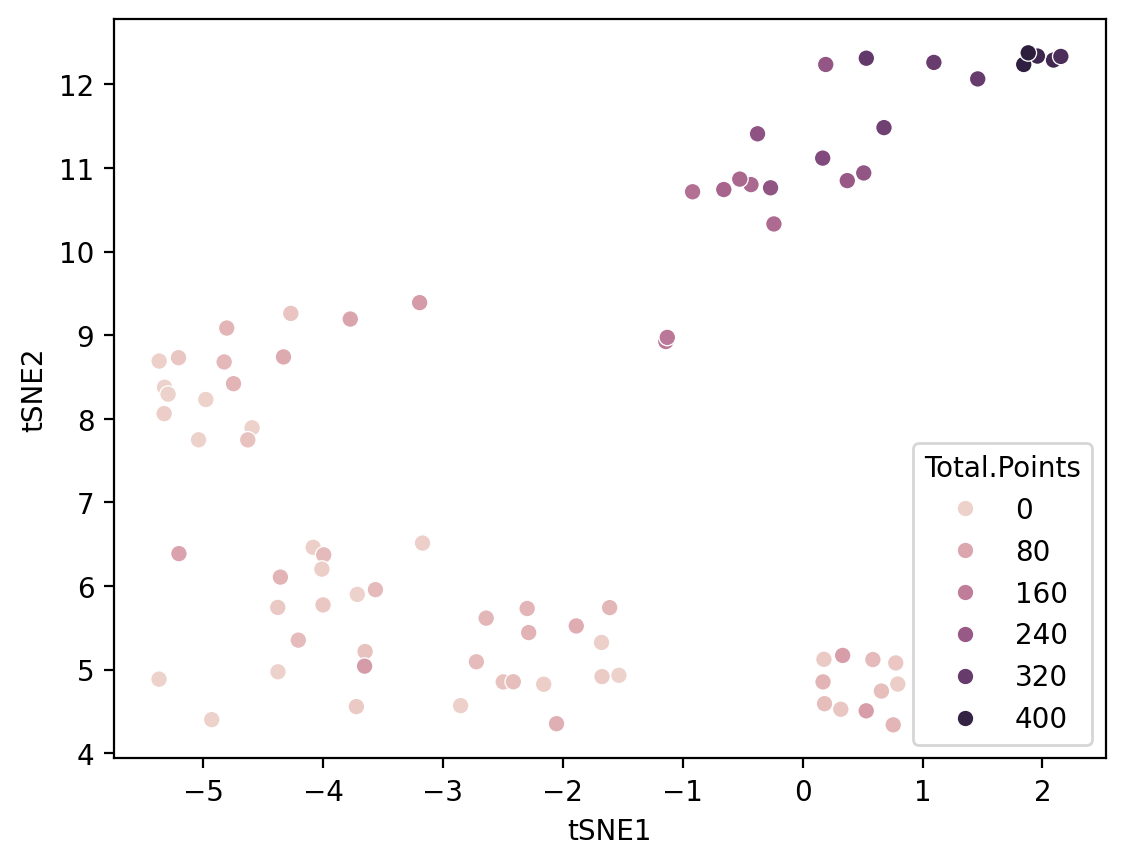
\includegraphics[width=\textwidth]{tsne_plot.png}
    \caption{Διάγραμμα Διασποράς t-SNE}
    \label{fig:tsne}
\end{figure}

\section{Εφαρμογές Μηχανικής Μάθησης}
Το σύνολο δεδομένων χρησιμοποιήθηκε για καθήκοντα τόσο ταξινόμησης όσο και ομαδοποίησης.

\subsection{Ταξινόμηση}
Ένας ταξινομητής λογιστικής παλινδρόμησης εκπαιδεύτηκε στα δεδομένα. Το σύνολο δεδομένων χωρίστηκε σε σύνολα εκπαίδευσης και δοκιμών, και η απόδοση του ταξινομητή αξιολογήθηκε χρησιμοποιώντας μετρικές ακρίβειας και πίνακα σύγχυσης.

\subsection{Ομαδοποίηση}
Η ομαδοποίηση K-Means εφαρμόστηκε στο σύνολο δεδομένων. Οι ομάδες απεικονίστηκαν χρησιμοποιώντας τις συνιστώσες του PCA.

\begin{figure}[h]
    \centering
    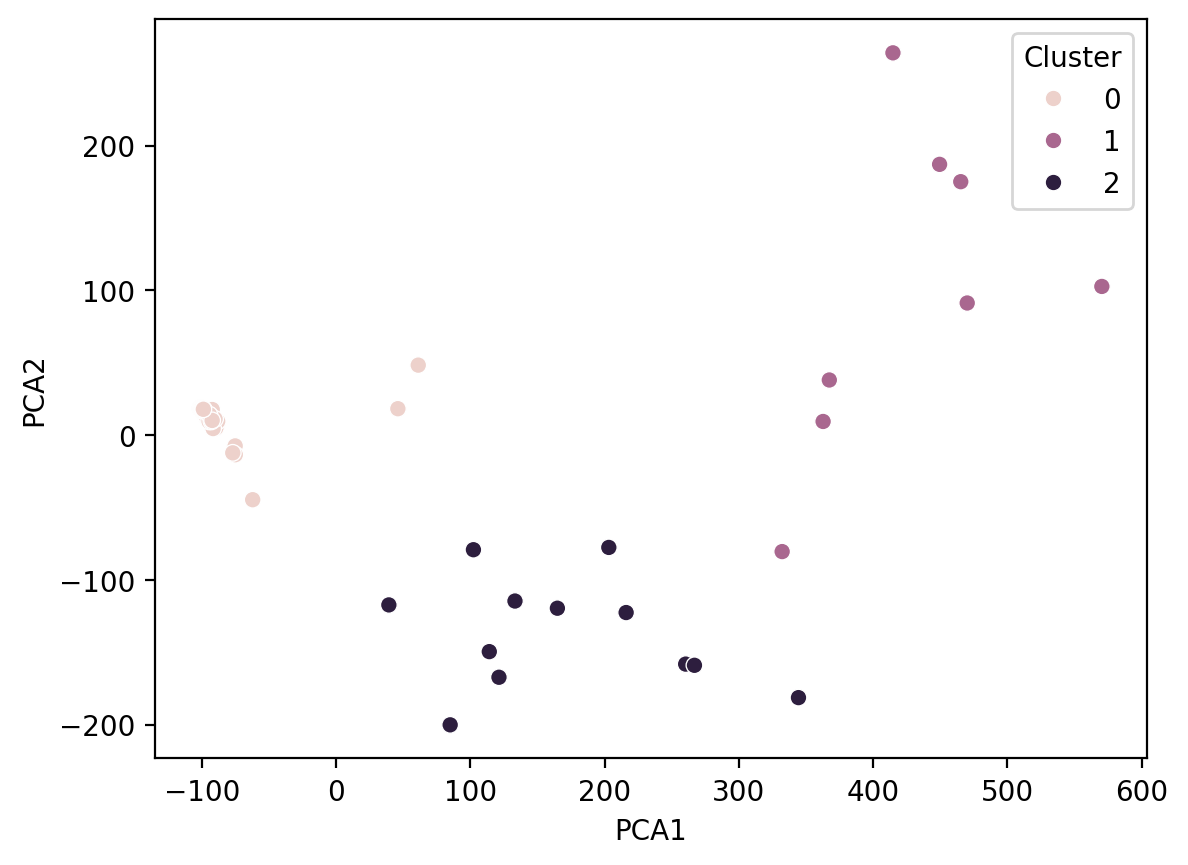
\includegraphics[width=\textwidth]{kmeans_plot.png}
    \caption{Διάγραμμα Ομαδοποίησης K-Means}
    \label{fig:kmeans}
\end{figure}

\section{UML Διάγραμμα}
Το παρακάτω διάγραμμα UML απεικονίζει την αρχιτεκτονική της εφαρμογής και της διεπαφής χρήστη. 

\begin{figure}[h!]
    \centering
    \includegraphics[width=\textwidth]{uml_diagram.png}
    \caption{UML Διάγραμμα Αρχιτεκτονικής Εφαρμογής και Διεπαφής Χρήστη}
    \label{fig:uml_diagram}
\end{figure}

\section{Κύκλος Ζωής Έκδοσης Λογισμικού}
Για την ανάπτυξη της εφαρμογής μας, ακολουθήσαμε το μοντέλο Agile. Το Agile είναι ένα επαναληπτικό και προοδευτικό μοντέλο ανάπτυξης λογισμικού που υποστηρίζει την ταχεία προσαρμογή στις αλλαγές και την συνεχή βελτίωση.

\subsection{Σχεδιασμός}
Η ανάπτυξη ξεκίνησε με τη συλλογή απαιτήσεων και τον αρχικό σχεδιασμό της αρχιτεκτονικής του συστήματος. 

\subsection{Υλοποίηση}
Η υλοποίηση έγινε σε μικρούς επαναληπτικούς κύκλους (sprints), κάθε ένας από τους οποίους περιλάμβανε τον σχεδιασμό, την ανάπτυξη, τη δοκιμή και την ανατροφοδότηση.

\subsection{Δοκιμή}
Μετά από κάθε sprint, πραγματοποιούνταν δοκιμές για να διασφαλιστεί ότι οι νέες λειτουργίες λειτουργούν όπως αναμένεται και ότι δεν εισήχθησαν νέα σφάλματα.

\subsection{Έκδοση}
Η τελική έκδοση του λογισμικού δημοσιεύτηκε μετά από πολλαπλές επαναλήψεις, διασφαλίζοντας τη σταθερότητα και την αξιοπιστία του προϊόντος.

\subsection{Συνεχής Βελτίωση}
Μετά την έκδοση, συνεχίζουμε να παρακολουθούμε και να βελτιώνουμε την εφαρμογή, συλλέγοντας ανατροφοδότηση από τους χρήστες και προσαρμόζοντας το προϊόν στις ανάγκες τους.

\section{Συμπεράσματα}
Η ανάλυση δεδομένων Formula 1 με τη χρήση των παραπάνω τεχνικών παρείχε ενδιαφέροντα αποτελέσματα. Η PCA και το t-SNE επέτρεψαν την οπτικοποίηση της δομής των δεδομένων, ενώ οι μέθοδοι ταξινόμησης και ομαδοποίησης έδωσαν σημαντικά αποτελέσματα για την κατηγοριοποίηση και την ομαδοποίηση των δεδομένων.

\section{Ομάδα Ανάπτυξης}
Στο πλαίσιο της εκπόνησης της εργασίας στο μάθημα «Τεχνολογίες Λογισμικού» τα μέλη της ομάδας συνεργάστηκαν και εκτέλεσαν τα ζητούμενα της εργασίας ισόποσα. Το έργο αναπτύχθηκε από:
\begin{itemize}
    \item Παύλος - Μάριος Γιαννάκος 
    \item Σταμάτης Πέτρου
\end{itemize}

\end{document}
